
\section{RQ2. To what extent are the artifically generated variants different?}

In this second research question, we investigate to what extent the artificially created variants are different between them and to the original program. To conduct this research question, we could separate the question in three fields as \autoref{diagrams:protocol:rq2} illustrates: static comparison, variant's preservation and  dynamic comparison. The three fields are addressed in the CROW and MEWE contributions.
The static analysis focuses on the appreciated differences between the program variants between them and against the original program. The preservation study highlight the fact that \wasm still is an intermediate code and compilers can undo code transformations from previous stages, therefore, it is important to conduct a study on how this transformations are maintained through \wasm programs' lifecycle, from their creation to the machine code execution.
All that said, in this work we focus on the last category, the dynamic analysis of the generated variants. This decision is supported due to that dynamic side-channels are offered through the execution of \wasm and we want to go deeper in this analysis.
We use the original functions from corpora described in \autoref{section:crow:corpora} and their variants generated in the answering of RQ1. 

\begin{figure*}[h]
    \centering
    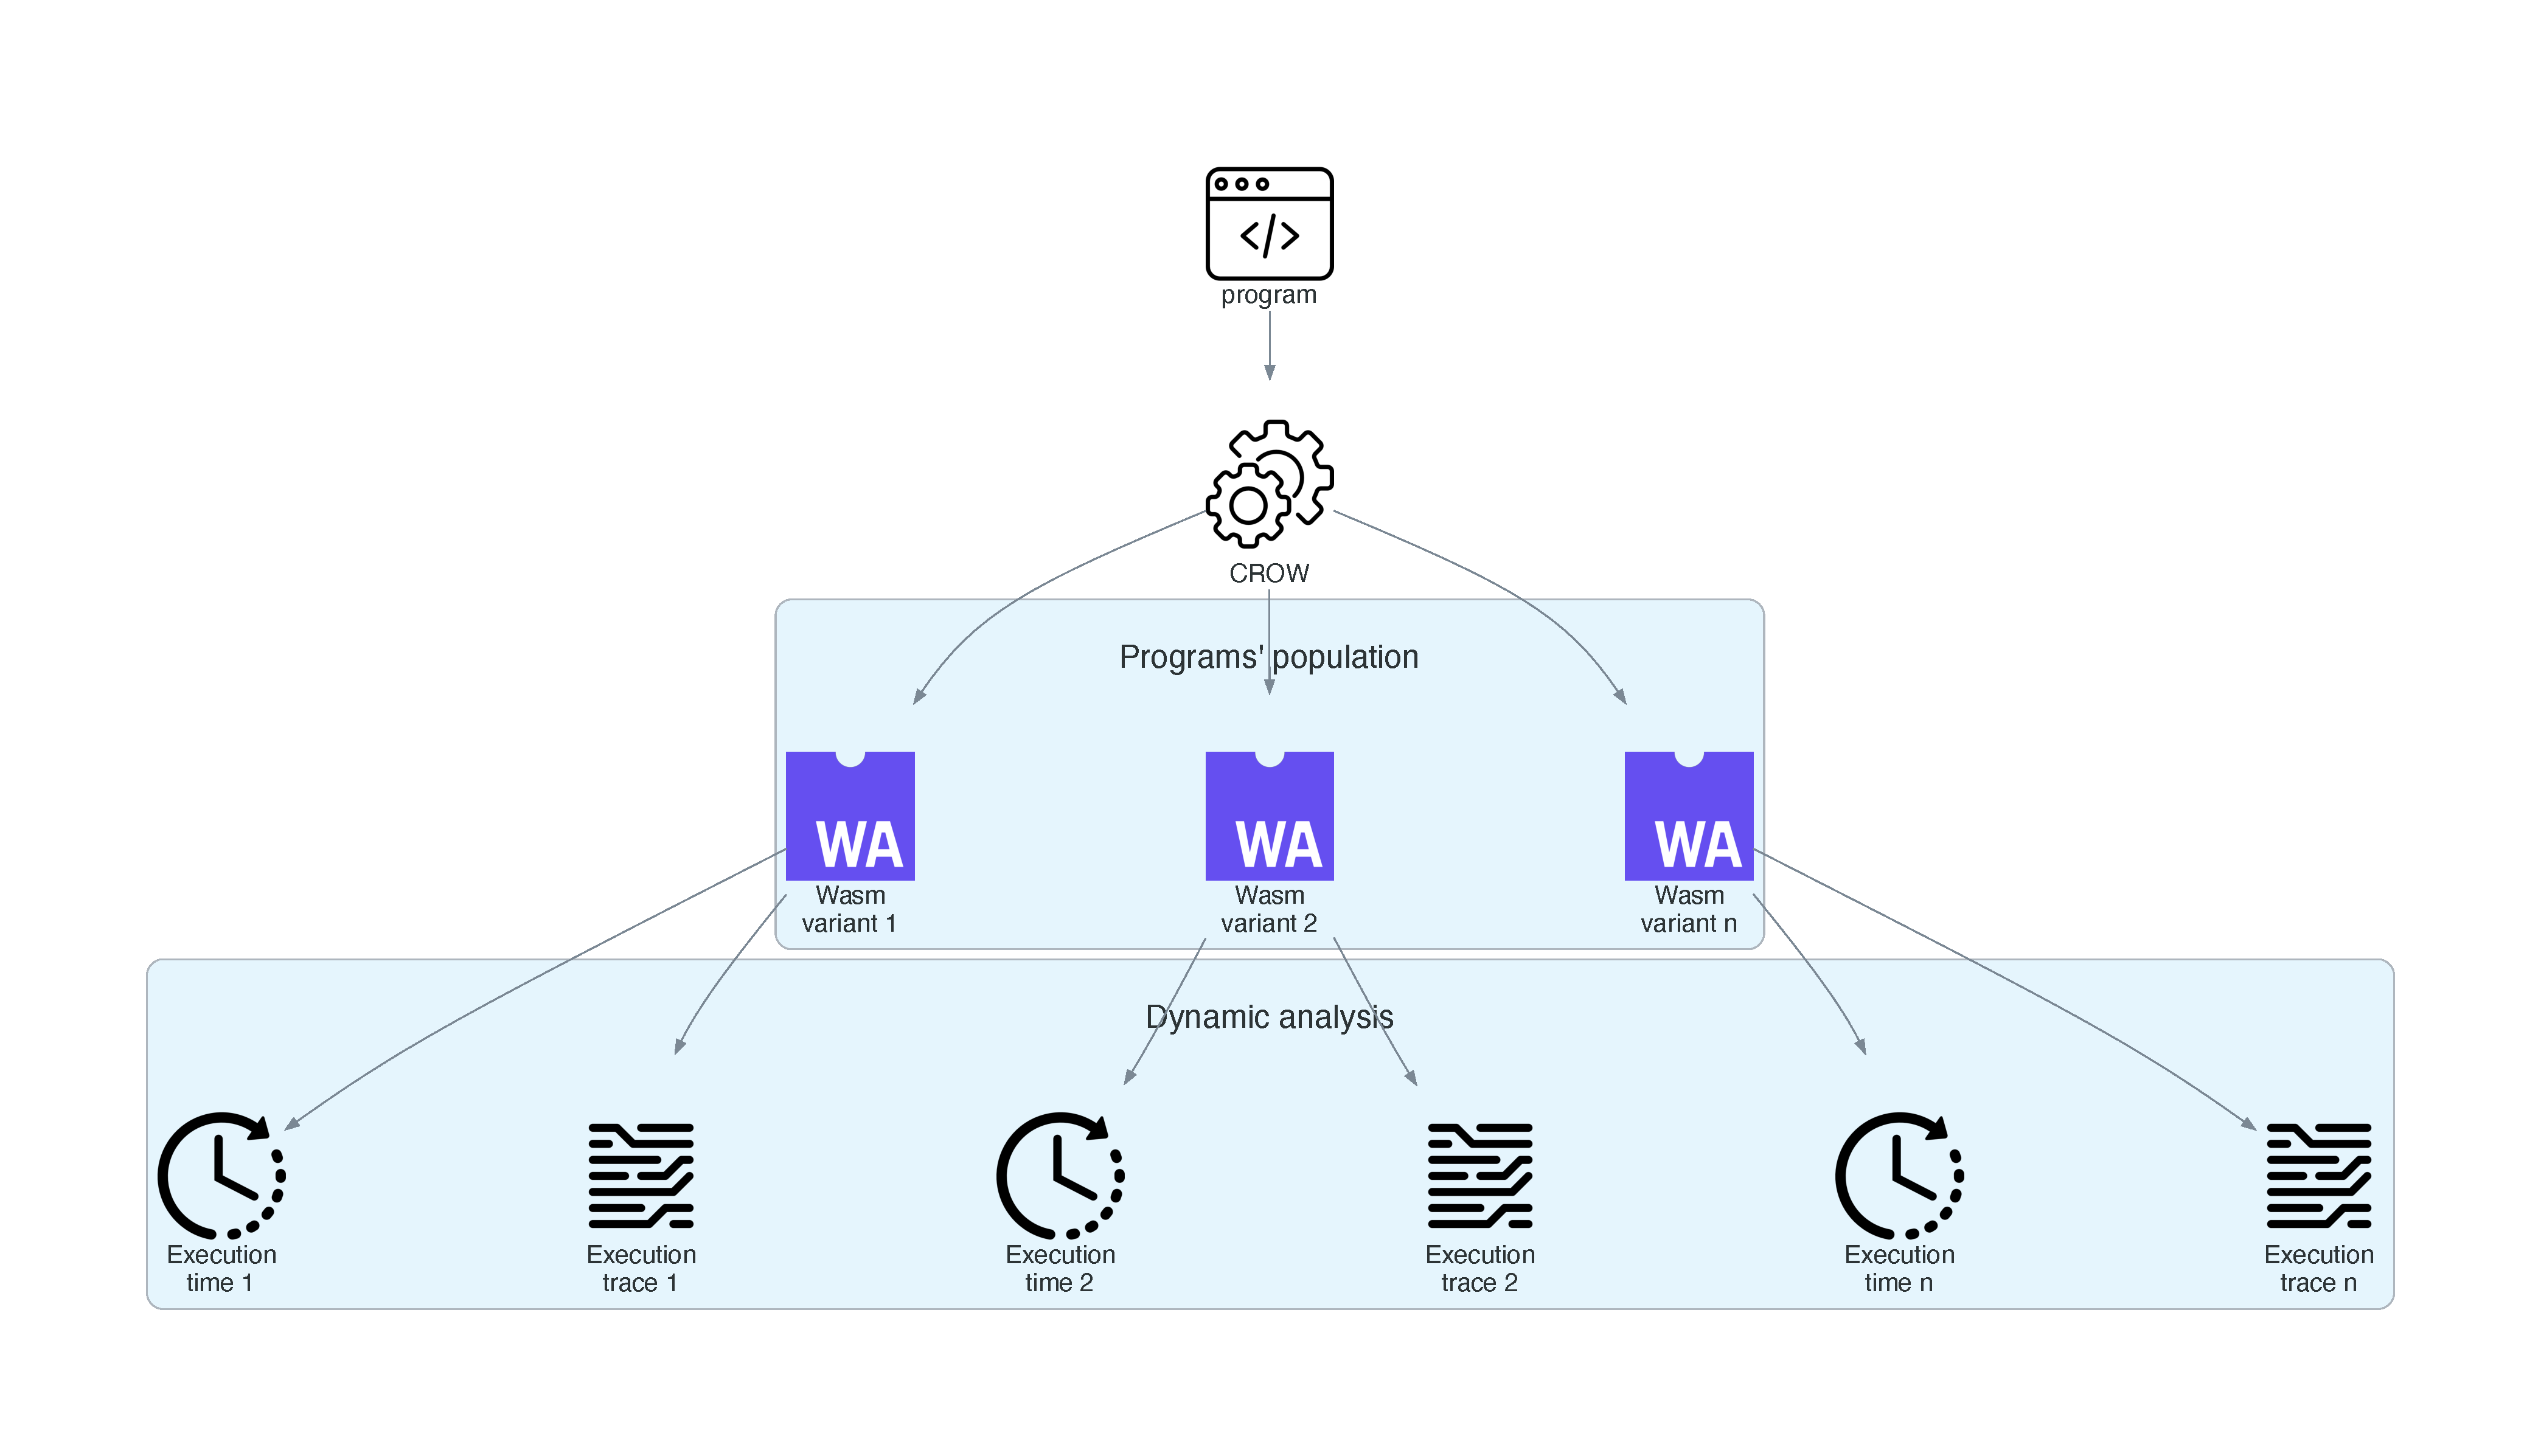
\includegraphics[height=3in]{diagrams/Rq2.pdf}
    \caption{Population study methodology for each original corpora and the variants generated in RQ1.}
    \label{diagrams:protocol:rq2}
\end{figure*}

We execute each program on each population to collect their execution traces and execution times. Furthermore, we then compare their dynamic behavior. We perform fine-grained comparisons by studying all pairs of programs in the population. Therefore, all defined metrics are formulated to support a pairwise comparison strategy.
In the following, we define the metrics used to answer RQ2.

\subsection{Metrics}

We measure the difference between programs at runtime by comparing their execution times and execution traces. We compare their execution traces with an alignment metric at the function and instruction level. Concretely, we propose a global alignment approach using Dynamic Time Warping (DTW) for their execution traces. In previous work, we highlighted how this approach measure similarity \citationneeded. 
Dynamic Time Warping \cite{Maia08usinga} computes the global alignment between two sequences. It returns a value capturing the cost of this alignment, which is a distance metric. The larger the DTW distance, the more different the two sequences are.
In the following, we define the $\DTW$ metric. 
 
\begin{comment}

\begin{metric}{dt\_static:}
    \label{metric:static1}
	Given two programs of the same program's population $P_X$ and $V_X$ written in $X$ code, dt\_static($P_X$, $V_X$), computes the DTW distance between the corresponding program instructions for representation $X$. \\
	
	A dt\_static($P_X$, $V_X$) of $0$ means that the code of both the original program and the variant  is the same, i.e., they are statically identical in the representation $X$. The higher the value of dt\_static, the more different the programs are in representation X. \\

	Notice that, for comparing \wasm programs, the metric is the instantiation of \DTWStatic with $X=WebAssembly$.
\end{metric}

\end{comment}

\begin{metric}{\DTW{}:}
\label{metric:stack}
	Given two programs P and P' from the same program's population and $T$ a trace space \DTW{}(P,P',T), computes the DTW distance between the traces collected during their execution in the $T$ space. A \DTW{} of $0$ means that both traces are identical. \\ 
	
	The higher the value, the more different the traces. 
\end{metric}

\begin{metric}{Execution time:}\label{metric:time}
	Given a \wasm program P, the execution time is the time spent to execute the binary.
\end{metric}

Notice that, for \autoref{metric:stack} we mentioned $T$ as a trace space. $T$ represents a topology over two types of traces, the function call stack and the virtual stack operations. A trace for the function call stack is the consecutive list of all functions called during the execution of the \wasm program. The virtual stack trace is the consecutive list of \texttt{push} and \texttt{pop} operations performed by the \wasm engine during the execution of the program.

%\subsection{Variants preservation}


\wasm is an intermediate language, and interpreters produce machine code to execute them. For program variants, this means that compiling can undo artificially introduced transformations, for example, through optimization passes. When a code transformation for a variant is maintained from the first time it is introduced to the final machine, code generation is then a preserved variant. For this mentioned reasoning, we need a preservation metric. The critical property we consider is as follows:


% In

\begin{property}{Preservation:}
	\label{property:preservation}
	Given a program P and a variant V' from the same program's population, if \DTWStatic{}($P_{Wasm}$, $P_{Wasm}'$) $>$ 0 and \DTWStatic{}($P_{x86}$, $P_{x86}'$) $>$ 0 $\implies$  both programs are still different when compiled to machine code.
	
	If the property fits for two programs, then the underlying compiler does not remove the transformations made by \tool. 
\end{property}


\begin{metric}{Preservation:}\label{metric:preservation}
	Given a \wasm programs P and a collection of generated variants $V$, the preservation ratio is the number of pair of programs that fit with \autoref{property:preservation} for a specific compiling engine over the total number of program pairs.
\end{metric}

\subsection{Protocol}

% One paragraph per metric
% Static
For each program's population generated in answering RQ1, we compare the sequence of instructions of each variant with the initial program and the other variants. We obtain the \autoref{metric:static1} values for each program-variant \wasm pair code. 

% Dynamic
To compare program and variants behavior during runtime, we analyze all the unique program variants generated by \tool in a pairwise comparison. 
We use SWAM\footnote{\url{https://github.com/satabin/swam}} to execute each program and variant to collect the function and instruction traces. SWAM is a \wasm interpreter that provides functionalities to capture the dynamic information of \wasm program executions, including the virtual stack operations. 

Furthermore, we collect the execution time, \autoref{metric:time}, for all programs and their variants. We execute each program or variant 10000 times, and we compare the collected execution time distributions using a Mann-Withney test \citationneeded in a pairwise strategy.

We collect \autoref{metric:preservation} for all program pairs in all program populations. We use two \wasm engines to study variant's preservation after compiling.

\begin{itemize}
    \item \textbf{V8} \citationneeded: the engine used by Chrome and NodeJS to execute JavaScript and \wasm. 
    \item \textbf{wasmtime} \citationneeded: a standalone runtime for WebAssembly. This engine is used by the Fastly platform to provide Edge-Cloud computing services. 
\end{itemize}

We only consider the x86 representation after the \wasm code is compiled to the machine code. 
This decision is not arbitrary. According to a previous study \citationneeded, any conclusion carried out by comparing two program binaries under a specific target can be extrapolated to another target for the same binaries.

%Part of the contributions of this thesis are our strategies to prevent reversion of code transformations. We take engineering decision regarding this in all the stages of the CROW workflow. We disable all optimizations inside CROW in the generation of the \wasm binaries. This prevents the LLVM toolchain used to remove some introduced transformations. However, the LLVM toolchain applies optimizations by default, such as constant folding or logical operations' normalization. As we illustrate previously, these are some transformations found and applied by CROW. We modified the LLVM backend for \wasm to avoid this reversion during the creation of Wasm binaries.
%This phenomenon is sometimes bypassed by diversification studies when they are conducted at high-level. As another contribution, we conduct a study on preservation for both scenarios where Wasm is used, browsers and standalone engines.

%\subsection{Setup}

